
\chapter{Results}

\acresetall


\section{Humanly Perceived Improvement vs. Machine Performance}


\subsection{Investigating Existing Data}

The direct comparison method outlined in \subsecref{Method-Existing-Data}
was carried out on the data given in \secref{litresults} \textit{\nameref{sec:litresults}}.
The R code used to perform this analysis is given in \lstref{directComp}.

\figref{Direct-PESQ-PRR} shows the results obtained, comparing the
\ac{PESQ} improvement against the \ac{PRR} improvement. \figref{Direct-PESQ-PRR-LOESS}
shows the data fitted with an \ac{LOESS} model and \figref{Direct-PESQ-PRR-LM}
shows the data fitted with an \ac{LM} method.

\begin{figure}[p]
\subfloat[\label{fig:Direct-PESQ-PRR-LOESS}\acs{LOESS} fit]{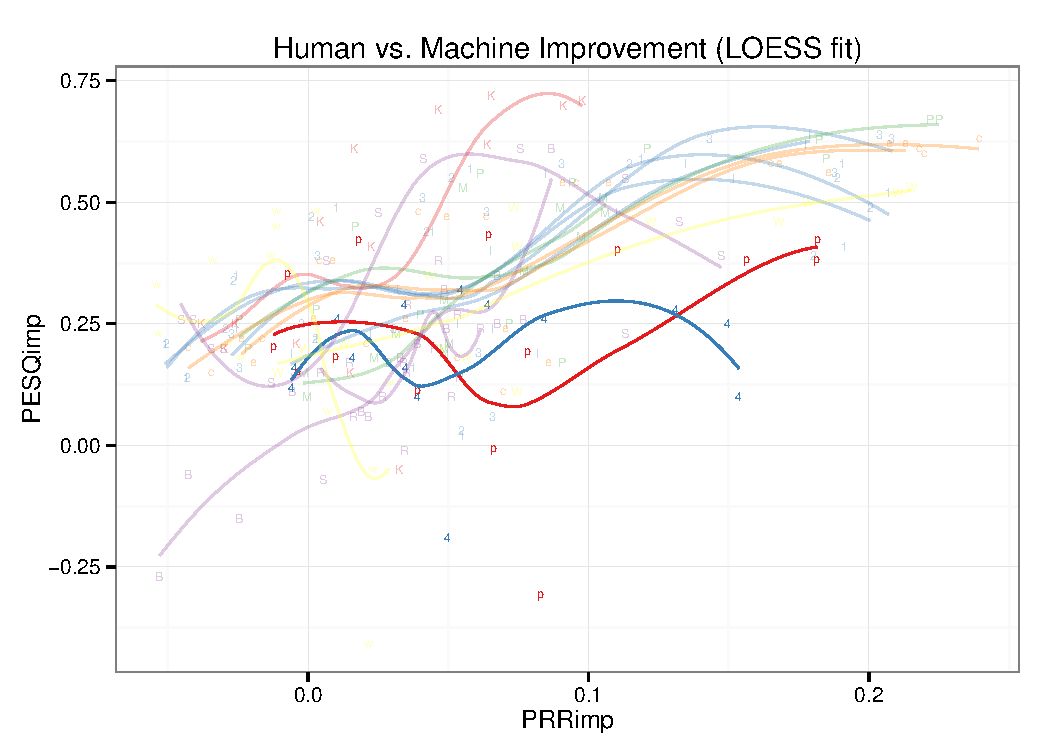
\includegraphics[width=1\textwidth]{fig/R/dir/lit/HumanMachineAllLOESS}

}

\subfloat[\label{fig:Direct-PESQ-PRR-LM}\acl{LM} fit]{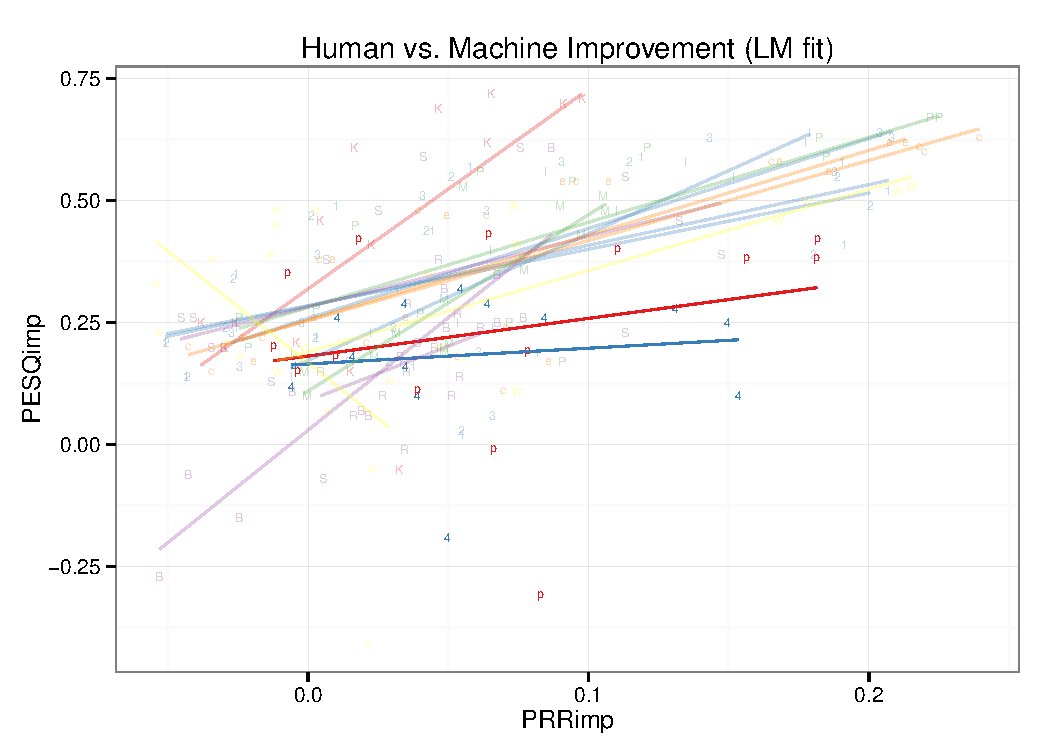
\includegraphics[width=0.8\textwidth]{fig/R/dir/lit/HumanMachineAllLM}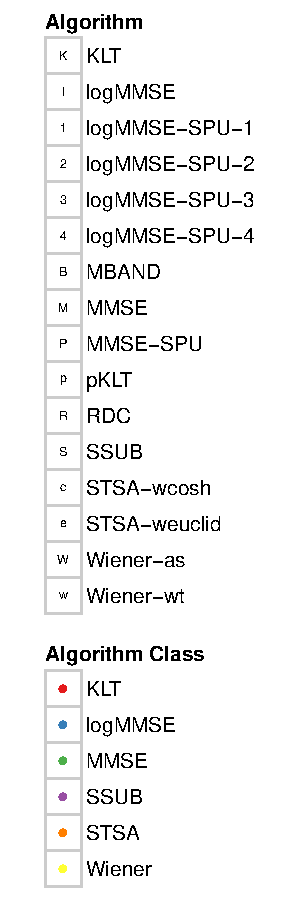
\includegraphics[width=0.2\textwidth]{fig/R/dir/lit/HumanMachineAllLegend}

}\protect\caption{\label{fig:Direct-PESQ-PRR}Direct comparison of human (\acs{PESQ})
vs. machine (\acs{PRR}) quality improvement}
\end{figure}


Additionally, a Pearson's correlation table was formed over a number
of the evaluation measures, depicted in the correlogram in \figref{litResCorr}.
The sparsity in this figure is due to the limited amount of pre-existing
data.

\begin{minipage}[t]{1\columnwidth}%
\begin{shaded}%

\subsubsection*{Correlograms}

A correlogram is a plot designed to allow the reader to quickly observe
the relationship between a number of variables. In the correlograms
included within this thesis, the leading diagonal shows the variable
name corresponding to that row and column. The upper panels display
a scatterplot where the y-axis represents the the variable of the
panel's row, and the x-axis represents the variable of the panel's
column. The lower panels show the Pearson's correlation of the two
variable the panel intersects, the 95\% confidence interval. Additionally,
lower panels are highlighted in red for negative correlations and
blue for positive correlations, with the darkness indicating magnitude.

So the darker shaded panels in the lower half indicate variables that
are strongly correlated, and allows the reader to quickly establish
which relationships are meaningful. The relationship can be visually
confirmed by checking the scatterplot in the upper half. The relationships
can then be further investigated by forming further plots of the variables
of interest.\end{shaded}%
\end{minipage}

\begin{figure}[h]
\noindent \begin{centering}
\includegraphics[width=1\textwidth]{fig/R/cor/litResCorrgram}
\par\end{centering}

\protect\caption{\label{fig:litResCorr}Correlogram of some of the evaluation measures
assessed in existing data}
\end{figure}


\clearpage{}


\subsection{Independent Investigation\label{sub:Independent-Investigation-Res}}

The following results correspond to algorithms listed in \tabref{Algorithms},
\textit{\nameref{tab:Algorithms}} and the evaluation measures outlined
in \subsecref{Independent-Investigation-Meth}, \textit{\nameref{sub:Independent-Investigation-Meth}}.
A correlogram of the results was formed in \figref{my-Corr} to give
an overview of the results and how measures correlated with one another.
In this figure:
\begin{itemize}
\item the \lstinline!utterances! and \lstinline!phonemes! rows/columns
correspond to the training given to the enhancement algorithm;
\item ``Imp'' refers to improvement comparatively with the signal before
enhancement, i.e., \lstinline!pesqImp! refers to the \ac{PESQ} score
after enhancement minus the \ac{PESQ} score before enhancement;
\item \lstinline!MOSle! refers to the \ac{MOS} listening effort scale
\citep{InternationalTelecommunicationUnion1996};
\item \lstinline!CMOS! refers to the comparative \ac{MOS};
\item \lstinline!PRRcorr! refers to the \ac{PRR} measured as the percentage
correct, or \ac{PRR} correctness;
\item \lstinline!PRRacc! refers the the \ac{PRR} measures as the accuracy,
defined as the number of correct phonemes minus the number of deletions,
substitutions and insertions, divided by the number of phonemes; and
\item \lstinline!segSNR! refers to the segmental \ac{SNR}.
\end{itemize}
The results for the various evaluation measures are given in \Cref{fig:my-PESQ,fig:my-PESQ-imp,fig:my-segSNR,fig:my-segSNR-imp,fig:my-PRRcorr,fig:my-MOS,fig:my-MOSle,fig:my-CMOS,fig:my-PRRcorr-imp,fig:my-PRRacc,fig:my-PRRacc-imp}.
These plots also show box plots of the five-point summaries of the
results. These results were used in investigating the correlation
between \ac{HR} and \ac{MR} and also to assess the performance of
the proposed changes to the enhancement algorithms outlined in \secref{Develop-Phoneme-Dependent}.
The changes proposed in \subsecref{Phoneme-Training} are implemented
in the algorithms \lstinline[breaklines=true]!phonemeIDBM!, \lstinline[breaklines=true]!phonemeMMSE!,
\lstinline[breaklines=true]!phonemeMohammadiaOnline! and \lstinline[breaklines=true]!phonemeMohammadiaSupervised!.
The changes proposed in \subsecref{Phoneme-Base} are implemented
in the algorithms \lstinline[breaklines=true]!phonemeModifiedOnline!
and \lstinline[breaklines=true]!phonemeModifiedSupervised!.


\subsubsection*{Observations}

During the \ac{MOS} tests, where it was noted that most participants
complained that occasionally a signal would not play. Upon further
investigation it was determined the signal was in fact playing, and
that the signal consisted of silence. Subjects were instructed to
continue answering the questions as they were worded, and thus these
signals were given the minimum scores. This is reflected in \Cref{fig:my-MOS,fig:my-MOSle,fig:my-CMOS},
where the ideal binary mask algorithms scored poorly.

\begin{figure}[h]
\noindent \begin{centering}
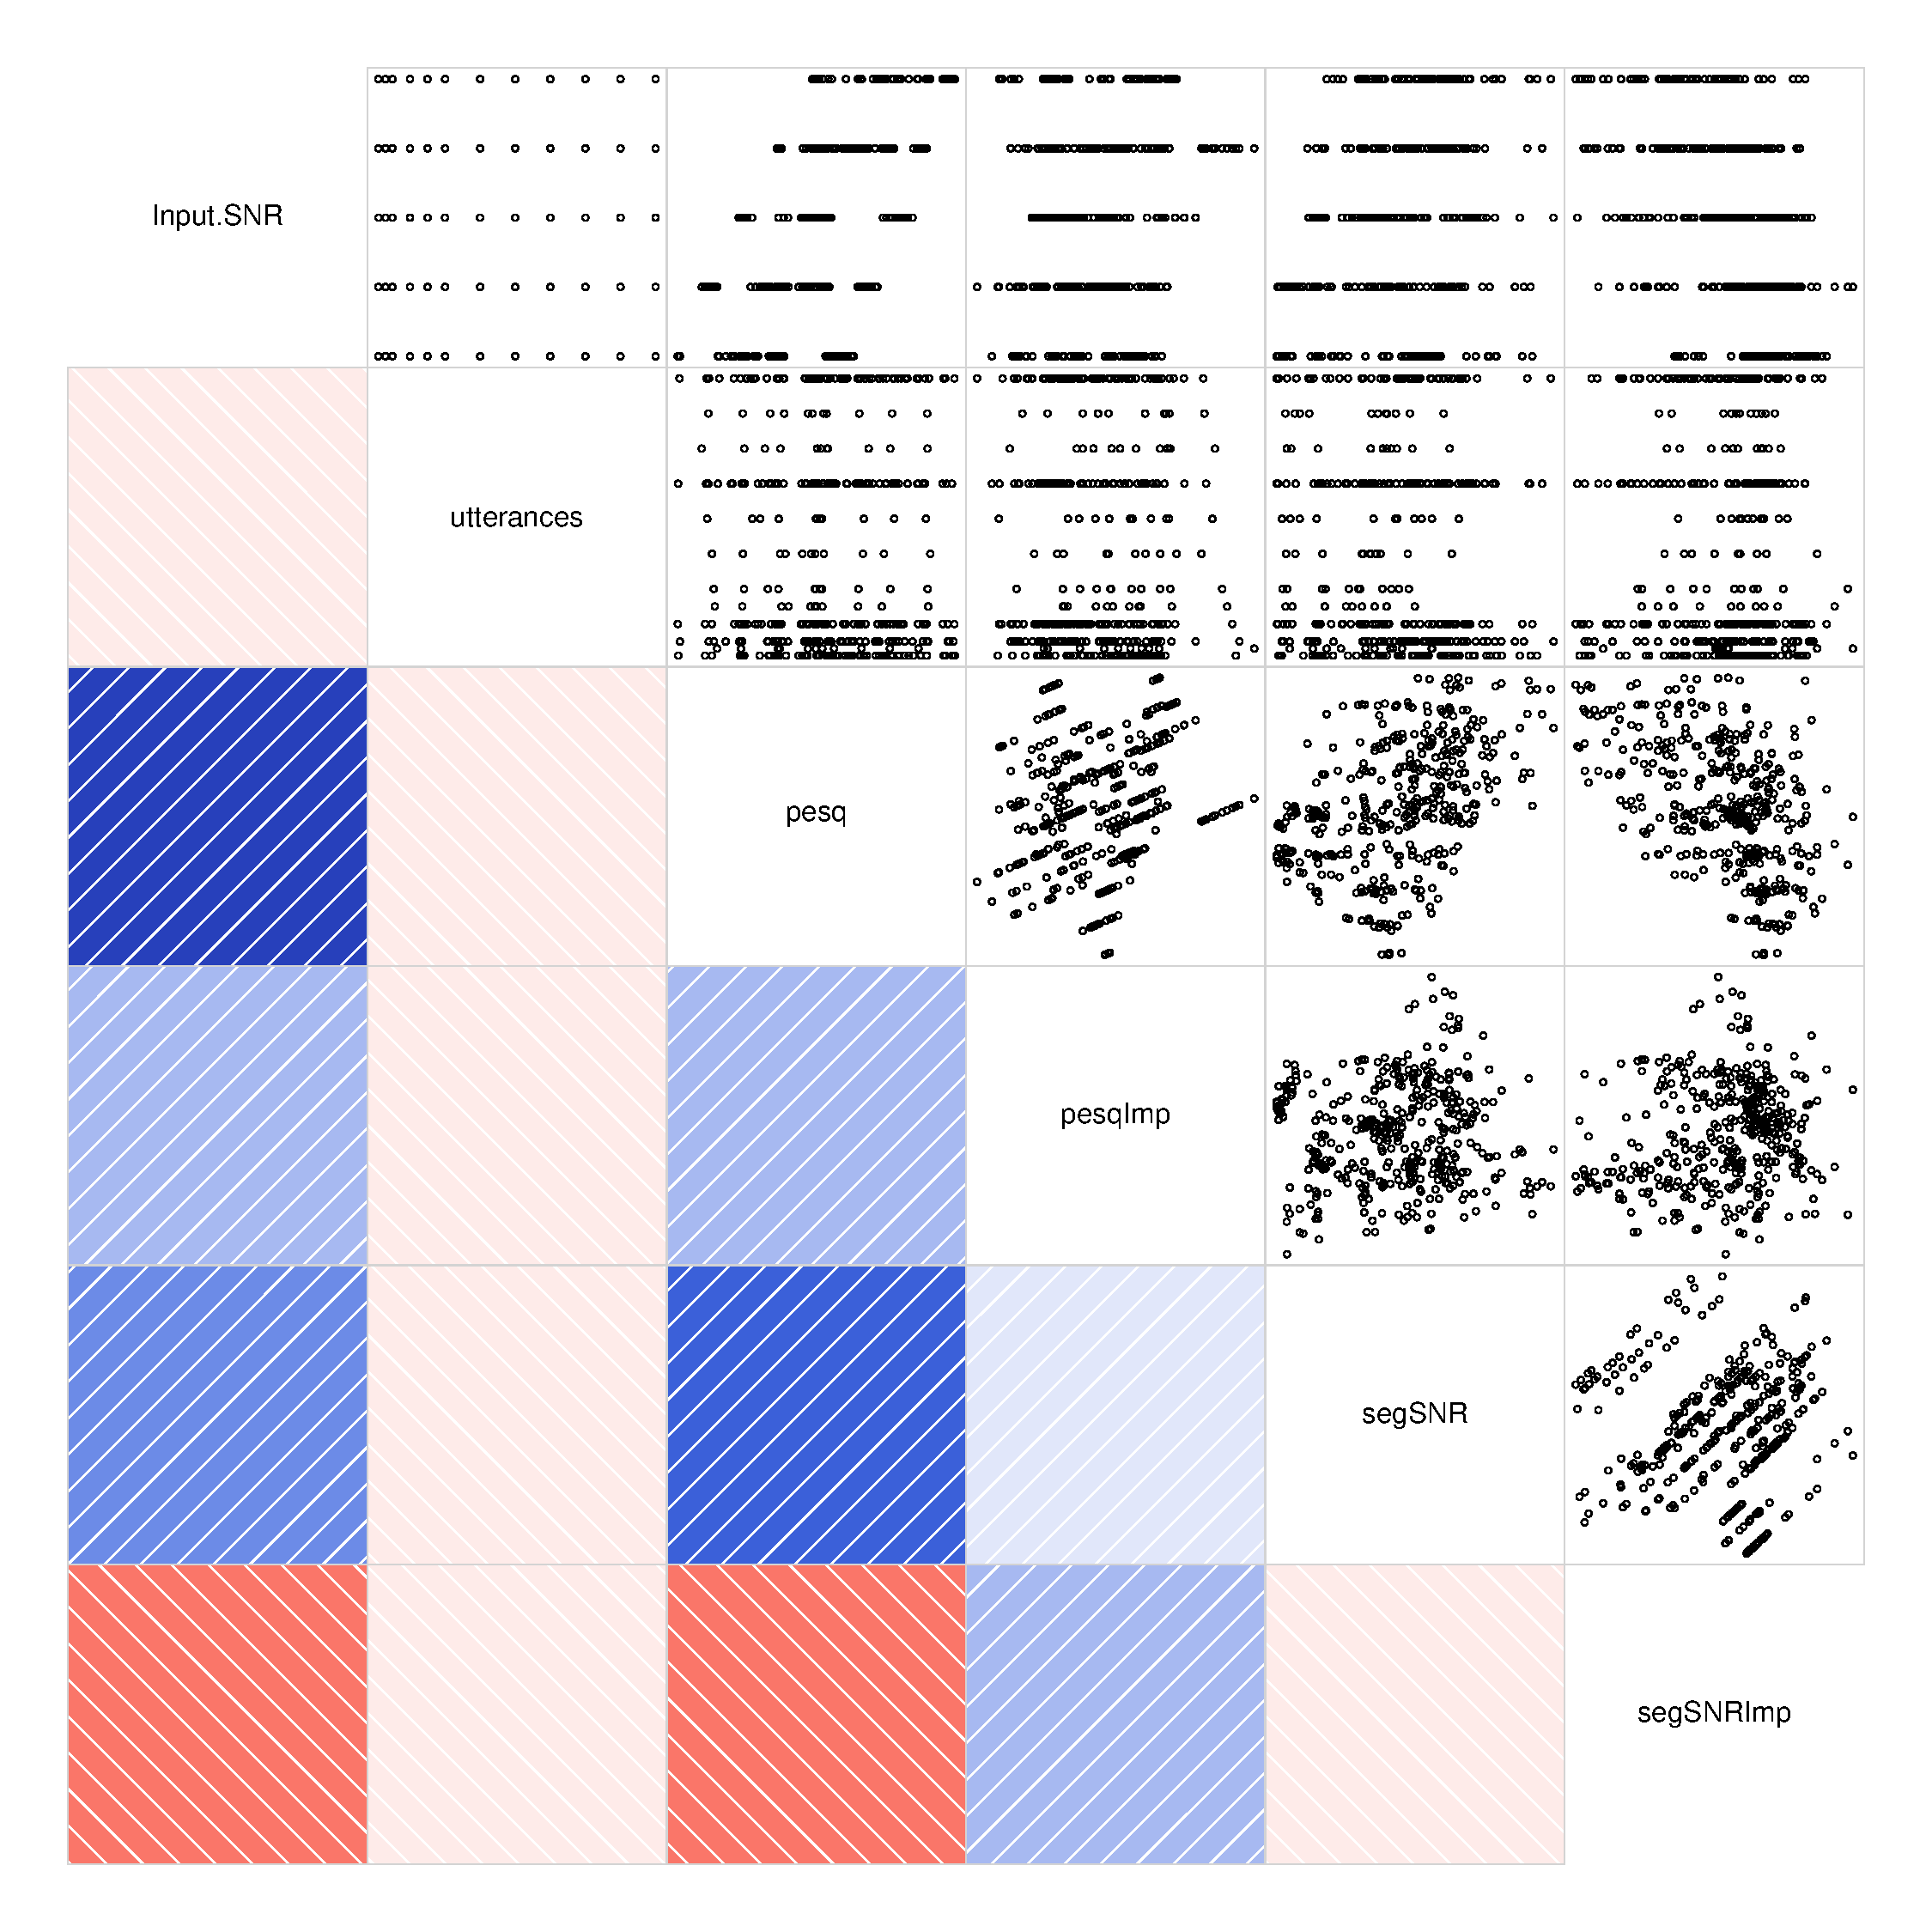
\includegraphics[width=1\textwidth]{fig/R/dir/my/corr}
\par\end{centering}

\protect\caption{\label{fig:my-Corr}Correlogram of results of independent investigation}
\end{figure}


\begin{figure}[p]
\noindent \begin{centering}
\includegraphics[angle=90,width=1\textwidth,height=0.95\textheight]{fig/R/my/pesq}
\par\end{centering}

\protect\caption{\label{fig:my-PESQ}\acs{PESQ} results of independent investigation}
\end{figure}


\begin{figure}[p]
\noindent \begin{centering}
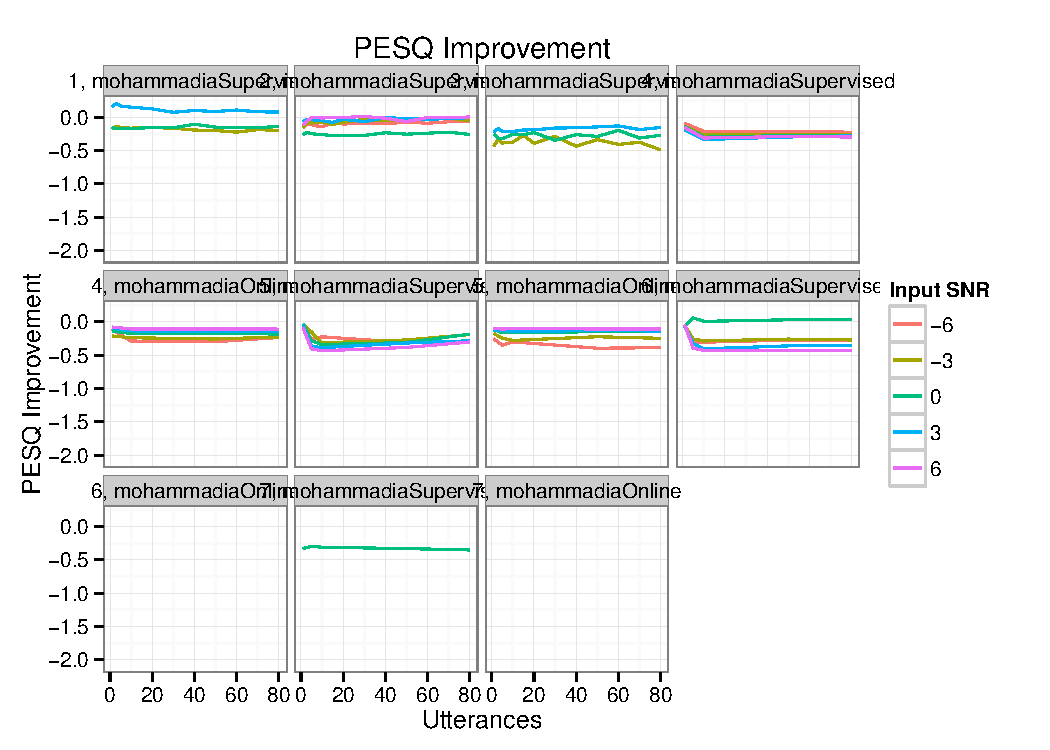
\includegraphics[angle=90,width=1\textwidth,height=0.95\textheight]{fig/R/my/pesqImp}
\par\end{centering}

\protect\caption{\label{fig:my-PESQ-imp}Improvement in \acs{PESQ} score due to enhancement}
\end{figure}


\begin{figure}[h]
\noindent \begin{centering}
\includegraphics[angle=90,width=1\textwidth,height=0.95\textheight]{fig/R/my/segSNR}
\par\end{centering}

\protect\caption{\label{fig:my-segSNR}Segmental \acs{SNR} results of independent
investigation}
\end{figure}


\begin{figure}[h]
\noindent \begin{centering}
\includegraphics[angle=90,width=1\textwidth,height=0.95\textheight]{fig/R/my/segSNRImp}
\par\end{centering}

\protect\caption{\label{fig:my-segSNR-imp}Improvement in segmental \acs{SNR} score
due to enhancement}
\end{figure}


\begin{figure}[h]
\noindent \begin{centering}
\includegraphics[angle=90,width=1\textwidth,height=0.95\textheight,keepaspectratio]{fig/R/my/MOS}
\par\end{centering}

\protect\caption{\label{fig:my-MOS}\acs{MOS} results of independent investigation}
\end{figure}


\begin{figure}[h]
\noindent \begin{centering}
\includegraphics[angle=90,width=1\textwidth,height=0.95\textheight,keepaspectratio]{fig/R/my/MOSle}
\par\end{centering}

\protect\caption{\label{fig:my-MOSle}Listening effort \acs{MOS} results of independent
investigation}
\end{figure}


\begin{figure}[h]
\noindent \begin{centering}
\includegraphics[angle=90,width=1\textwidth,height=0.95\textheight,keepaspectratio]{fig/R/my/CMOS}
\par\end{centering}

\protect\caption{\label{fig:my-CMOS}Comparative \acs{MOS} results of independent
investigation}
\end{figure}


\begin{figure}[h]
\noindent \begin{centering}
\includegraphics[angle=90,width=1\textwidth,height=0.95\textheight,keepaspectratio]{fig/R/my/PRRcorr}
\par\end{centering}

\protect\caption{\label{fig:my-PRRcorr}\acs{PRR} correctness results of independent
investigation}
\end{figure}


\begin{figure}[h]
\noindent \begin{centering}
\includegraphics[angle=90,width=1\textwidth,height=0.95\textheight,keepaspectratio]{fig/R/my/PRRcorrImp}
\par\end{centering}

\protect\caption{\label{fig:my-PRRcorr-imp}Improvement in \acs{PRR} correctness due
to enhancement}
\end{figure}


\begin{figure}[h]
\noindent \begin{centering}
\includegraphics[angle=90,width=1\textwidth,height=0.95\textheight,keepaspectratio]{fig/R/my/PRRacc}
\par\end{centering}

\protect\caption{\label{fig:my-PRRacc}\acs{PRR} accuracy results of independent investigation}
\end{figure}


\begin{figure}[h]
\noindent \begin{centering}
\includegraphics[angle=90,width=1\textwidth,height=0.95\textheight,keepaspectratio]{fig/R/my/PRRaccImp}
\par\end{centering}

\protect\caption{\label{fig:my-PRRacc-imp}Improvement in \acs{PRR} accuracy due to
enhancement}
\end{figure}


\clearpage{}


\section{Assessing \acl{NMF} Algorithm Training}

The following are the results of investigations attempting to answer
Research Question \ref{enu:ResQ2}, \textit{\RQtwo{}}


\subsection{Investigating Training Requirements}

The results of the experiments proposed in \subsecref{Investigating-Training-Req}
are given in this section. \Cref{fig:vary-train-pesq,fig:vary-train-mos,fig:vary-train-mosle,fig:vary-train-cmos,fig:vary-train-prrcorr,fig:vary-train-prracc,fig:vary-train-segsnr}
show the \ac{PESQ}, \ac{MOS}, \ac{MOS} listening effort, comparative
\ac{MOS}, \ac{PRR} correctness and \ac{PRR} accuracy results of
the \ac{BNMF} algorithm developed by \citet{mohammadiha2013supervised}
as a function of the number of utterances used in training.

Plots in \Cref{fig:vary-train-pesq,fig:vary-train-mos,fig:vary-train-mosle,fig:vary-train-cmos,fig:vary-train-prrcorr,fig:vary-train-prracc,fig:vary-train-segsnr}
each are arranged with the number of trained utterances on the x-axis
and test score on the y-axis. Furthermore, the plots are arranged
in a grid with rows corresponding to the enhancement algorithm and
columns corresponding to the test. Test labels give information on
the speaker ID and in brackets the sex of both the SoI, and the speakers
used to form the noise babble. Finally, series colour represents the
\ac{SNR} used for the test data, and the line type is dashed when
representing the score of the dirty signal before enhancement. The
R script used to form these plots is given in \lstref{trainReq}.

\begin{figure}[p]
\noindent \begin{centering}
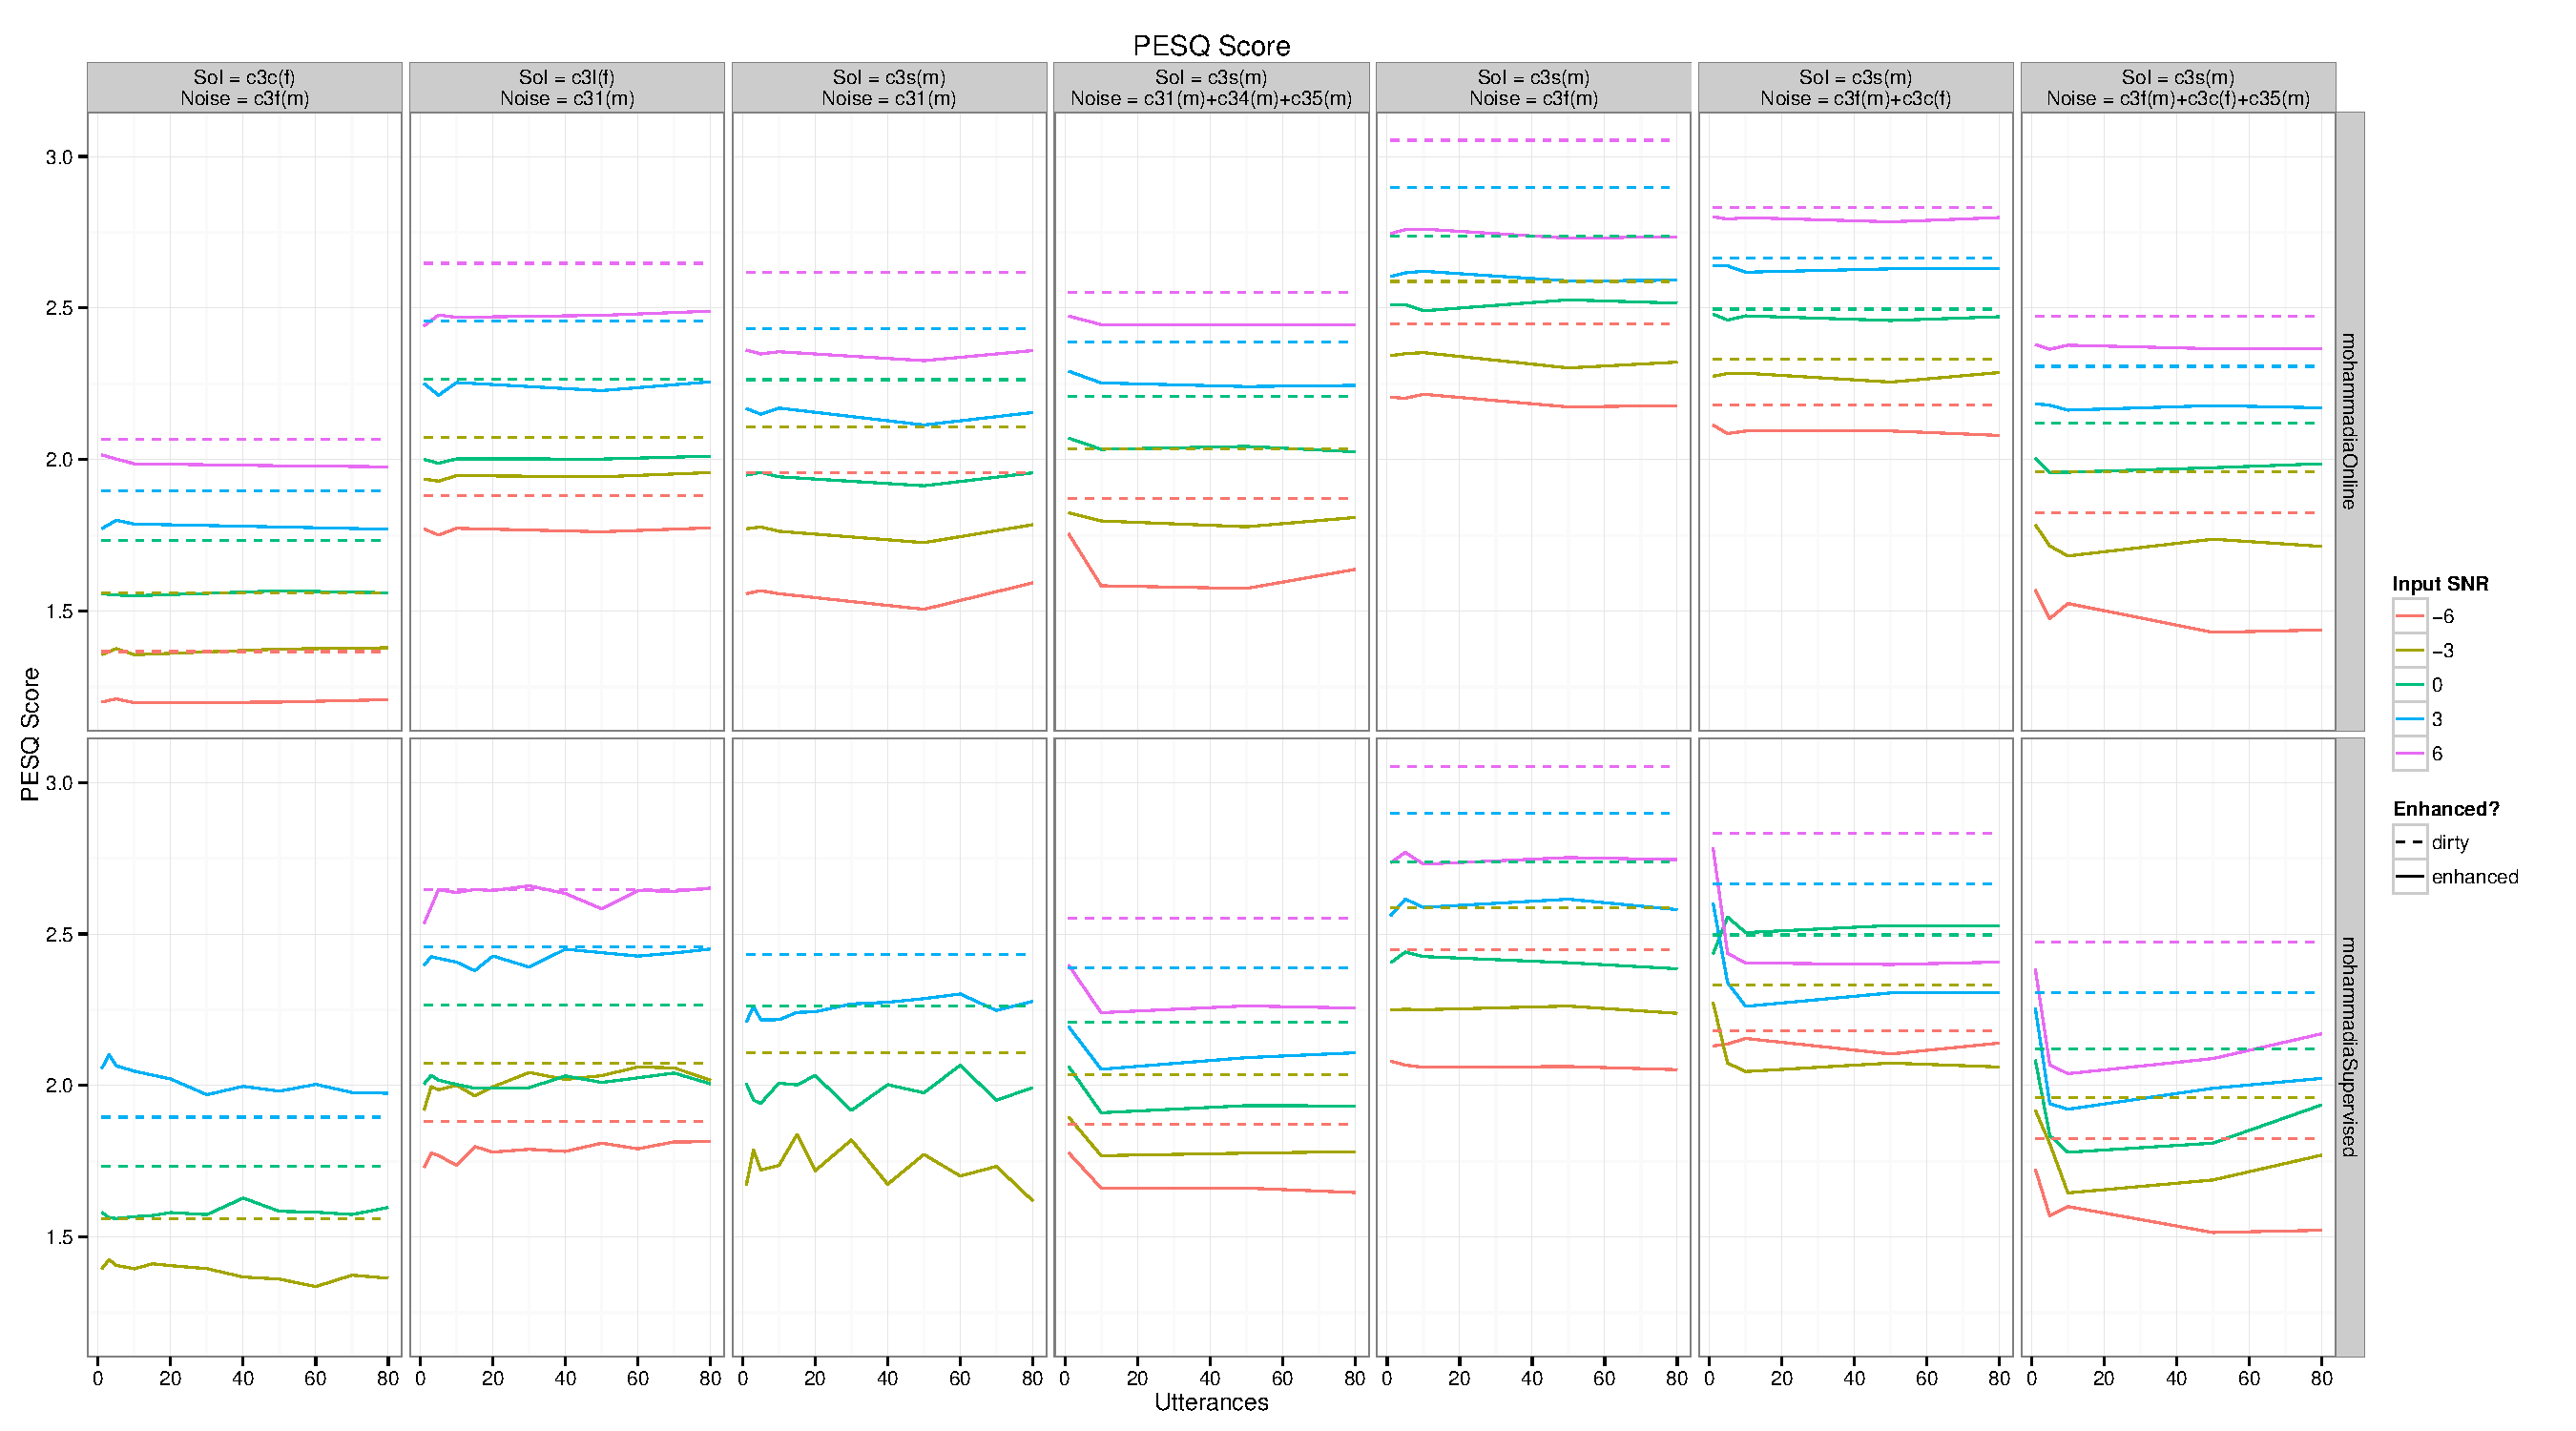
\includegraphics[angle=90,width=1\textwidth,height=0.95\textheight]{fig/R/train/pesq}
\par\end{centering}

\protect\caption{\label{fig:vary-train-pesq}\acs{PESQ} results of \acs{BNMF} algorithm
as training is increased}
\end{figure}


\begin{figure}[p]
\noindent \begin{centering}
\includegraphics[angle=90,width=1\textwidth,height=0.95\textheight,keepaspectratio]{fig/R/train/MOS}
\par\end{centering}

\protect\caption{\label{fig:vary-train-mos}\acs{MOS} results of \acs{BNMF} algorithm
as training is increased}
\end{figure}


\begin{figure}[p]
\noindent \begin{centering}
\includegraphics[angle=90,width=1\textwidth,height=0.95\textheight,keepaspectratio]{fig/R/train/mosle}
\par\end{centering}

\protect\caption{\label{fig:vary-train-mosle}\acs{MOS} listening effort results of
\acs{BNMF} algorithm as training is increased}
\end{figure}


\begin{figure}[p]
\noindent \begin{centering}
\includegraphics[angle=90,width=1\textwidth,height=0.95\textheight,keepaspectratio]{fig/R/train/CMOS}
\par\end{centering}

\protect\caption{\label{fig:vary-train-cmos}Comparative \acs{MOS} results of \acs{BNMF}
algorithm as training is increased}
\end{figure}


\begin{figure}[p]
\noindent \begin{centering}
\includegraphics[angle=90,width=1\textwidth,height=0.95\textheight,keepaspectratio]{fig/R/train/prrcorr}
\par\end{centering}

\protect\caption{\label{fig:vary-train-prrcorr} \acs{PRR} correctness results of
\acs{BNMF} algorithm as training is increased}
\end{figure}


\begin{figure}[p]
\noindent \begin{centering}
\includegraphics[angle=90,width=1\textwidth,height=0.95\textheight,keepaspectratio]{fig/R/train/prracc}
\par\end{centering}

\protect\caption{\label{fig:vary-train-prracc} \acs{PRR} accuracy results of \acs{BNMF}
algorithm as training is increased}
\end{figure}


\begin{figure}[p]
\noindent \begin{centering}
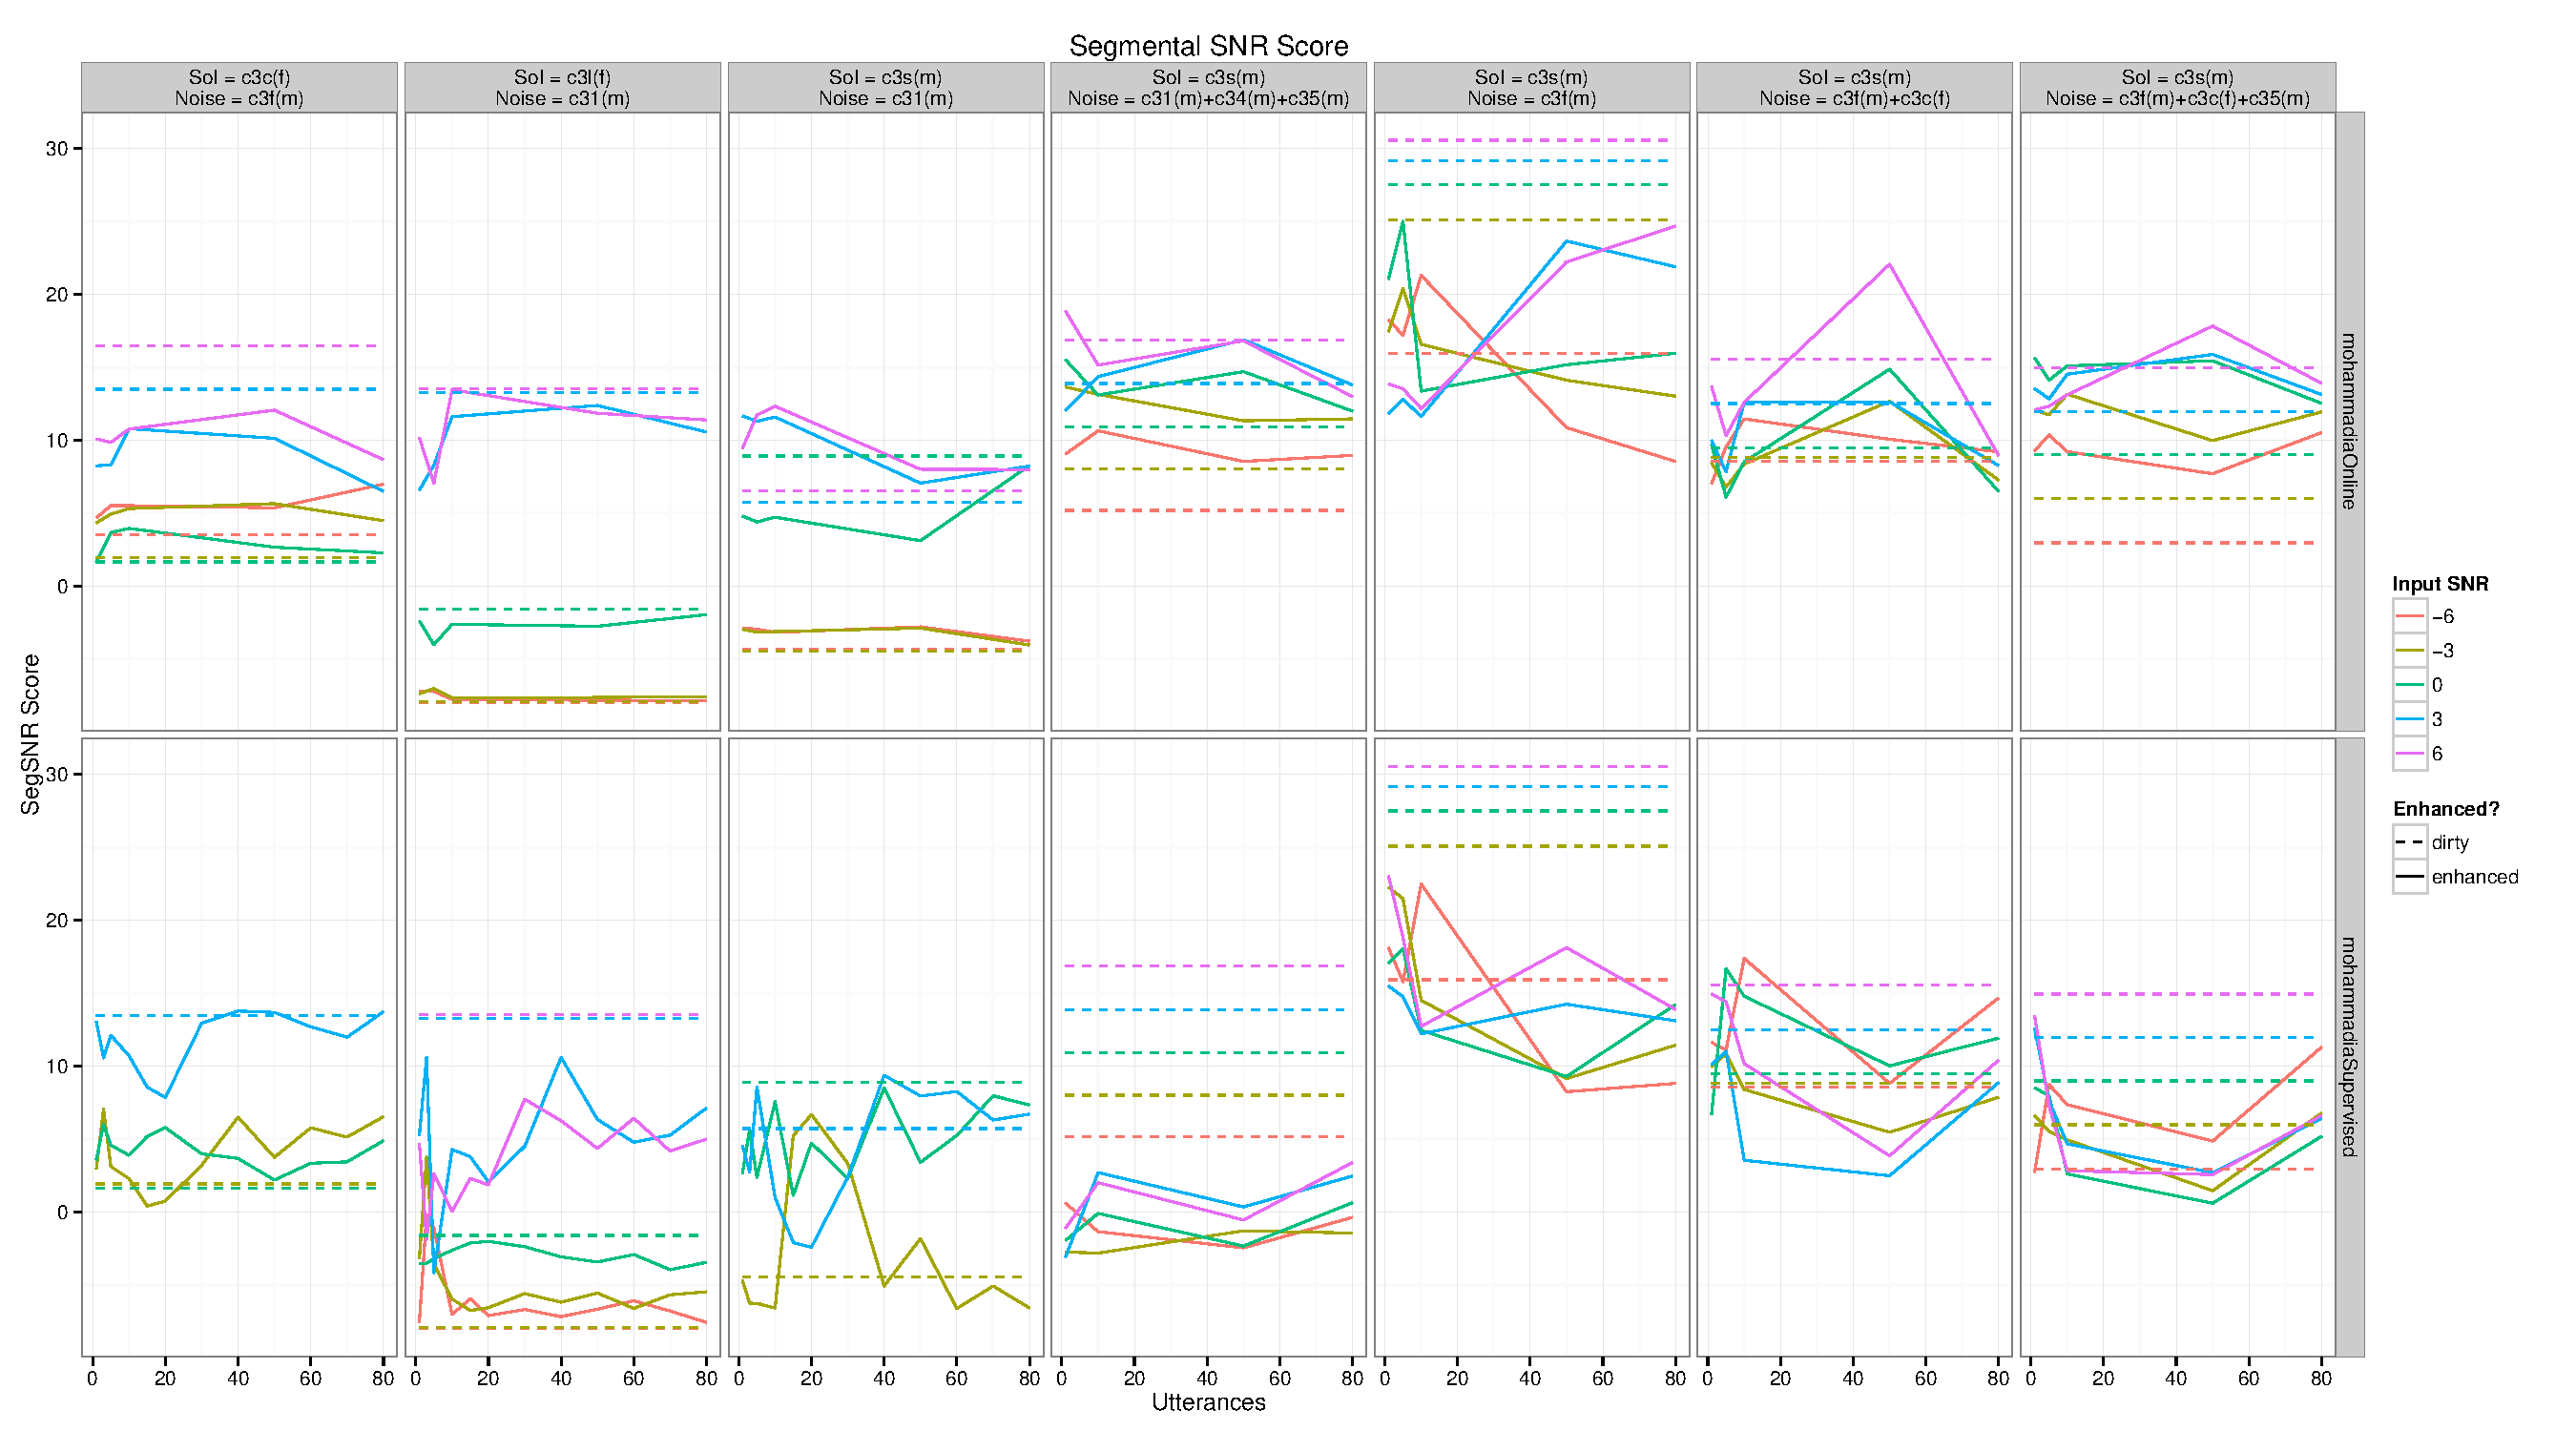
\includegraphics[angle=90,width=1\textwidth,height=0.95\textheight]{fig/R/train/segSNR}
\par\end{centering}

\protect\caption{\label{fig:vary-train-segsnr}Segmental \acs{SNR} results of \acs{BNMF}
algorithm as training is increased}
\end{figure}


\clearpage{}


\section{Phoneme-Dependent Variation Performance}

The results of the phoneme-dependent \textbf{training} algorithm proposed
in \subsecref{Phoneme-Training} and the phoneme-dependent \textbf{base}
algorithm proposed in \subsecref{Phoneme-Base} are given in this
section.

The typical spectrograms of the drawn phonemes are given in \figref{drawn-phoneme-spectrogram},
showing the frequency characteristics of each phoneme.

\begin{figure}[h]
\subfloat[\label{fig:mos-comparison-phn-1}One sample per phoneme]{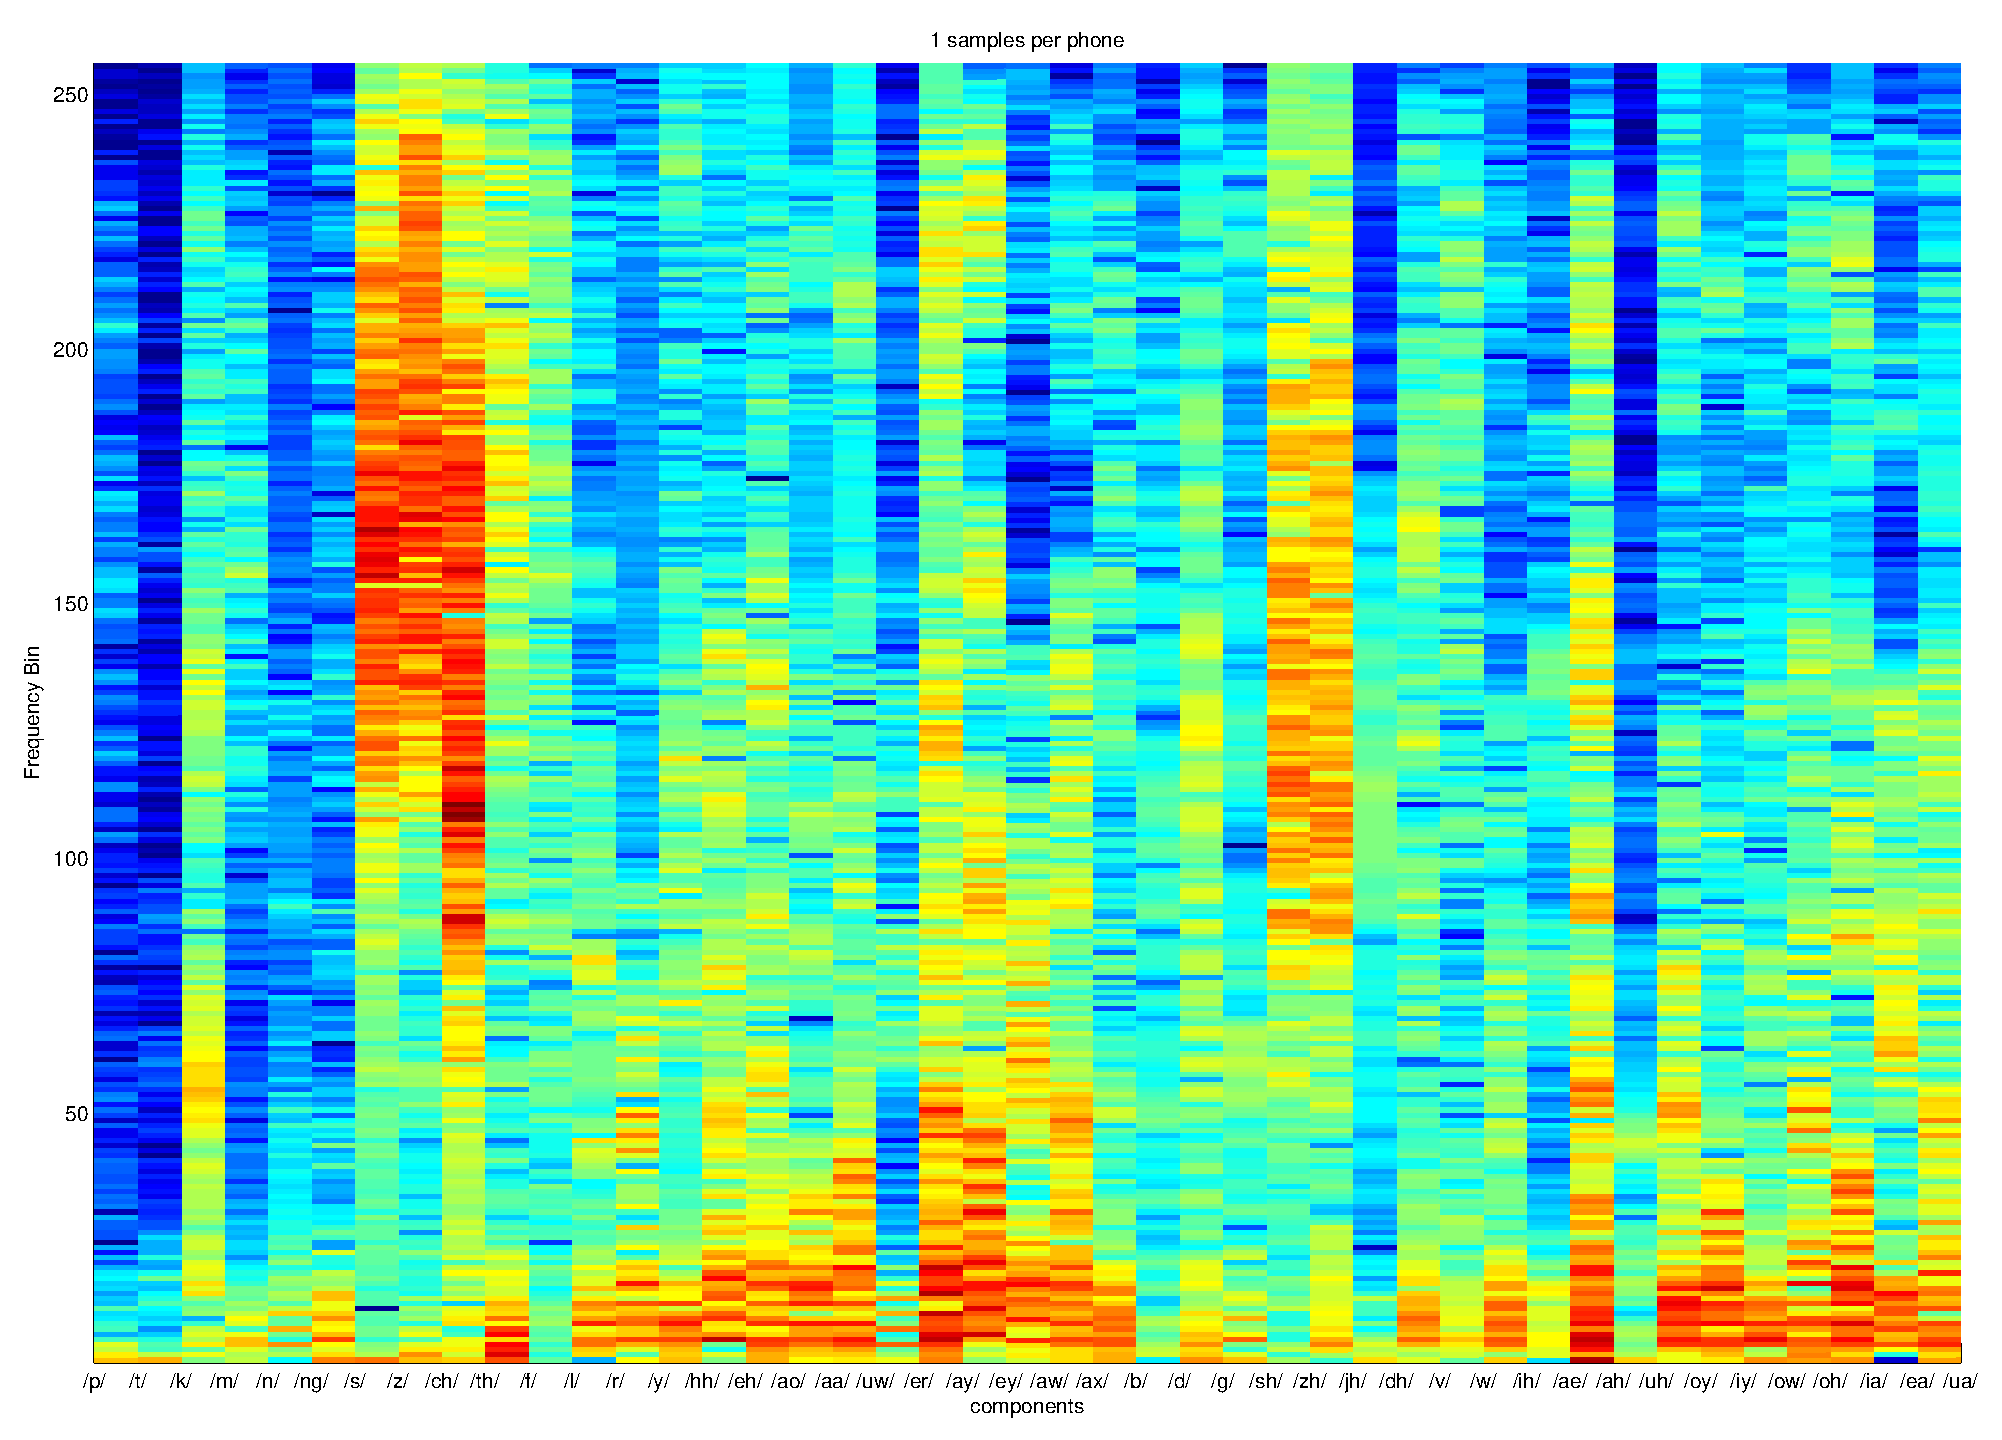
\includegraphics[width=0.5\textwidth]{fig/spectrogram/drawPhn/c3s-1phnSpectrogram}

}\subfloat[\label{fig:mos-comparison-phn-5}Five samples per phoneme]{

\includegraphics[width=0.5\textwidth]{fig/spectrogram/drawPhn/c3s-5phnSpectrogram}

}

\subfloat[Ten samples per phoneme]{\includegraphics[width=0.5\textwidth]{fig/spectrogram/drawPhn/c3s-10phnSpectrogram}

}\subfloat[50 samples per phoneme]{\includegraphics[width=0.5\textwidth]{fig/spectrogram/drawPhn/c3s-50phnSpectrogram}

}

\subfloat[100 samples per phoneme]{\includegraphics[width=0.5\textwidth]{fig/spectrogram/drawPhn/c3s-100phnSpectrogram}

}\subfloat[500 samples per phoneme]{\includegraphics[width=0.5\textwidth]{fig/spectrogram/drawPhn/c3s-500phnSpectrogram}

}

\subfloat[999 samples per phoneme]{\includegraphics[width=0.5\textwidth]{fig/spectrogram/drawPhn/c3s-999phnSpectrogram}

}

\protect\caption{\label{fig:drawn-phoneme-spectrogram}Typical spectrogram of randomly
drawn phoneme samples for speaker C3S}
\end{figure}


The performance of the phoneme-dependant algorithms have already been
given in \Cref{fig:my-PESQ,fig:my-PESQ-imp,fig:my-segSNR,fig:my-segSNR-imp,fig:my-PRRcorr,fig:my-MOS,fig:my-MOSle,fig:my-CMOS,fig:my-PRRcorr-imp,fig:my-PRRacc,fig:my-PRRacc-imp},
since these algorithms were also considered in the previous investigation.

Additionally given are plots comparing performance of algorithms without
modification against those with phoneme-dependent modification. These
are given in \Cref{fig:pesq-comparison-phn,fig:mos-comparison-phn,fig:mosle-comparison-phn,fig:cmos-comparison-phn,fig:prrcorr-comparison-phn,fig:prrcorrimp-comparison-phn,fig:prracc-comparison-phn,fig:prraccimp-comparison-phn,fig:segsnr-comparison-phn,fig:segsnrimp-comparison-phn}.
In these plots, the x-axis measures the performance of the original
algorithm, and the y-axis measures performance of the modified algorithm.
Therefore, any points lying above the diagonal line show better performance
for the modified algorithm, and below the line show better performance
for the original algorithm.

The phoneme dependent training data changes proposed in \subsecref{Phoneme-Training}
are implemented in the algorithms \lstinline[breaklines=true]!phonemeIDBM!,
\lstinline[breaklines=true]!phonemeMMSE!, \lstinline[breaklines=true]!phonemeMohammadiaOnline!
and\linebreak{}
\lstinline[breaklines=true]!phonemeMohammadiaSupervised! in \Cref{fig:my-PESQ,fig:my-PESQ-imp,fig:my-segSNR,fig:my-segSNR-imp,fig:my-PRRcorr,fig:my-MOS,fig:my-MOSle,fig:my-CMOS,fig:my-PRRcorr-imp,fig:my-PRRacc,fig:my-PRRacc-imp},
and are labelled ``Phoneme Training'' in \Cref{fig:pesq-comparison-phn,fig:mos-comparison-phn,fig:mosle-comparison-phn,fig:cmos-comparison-phn,fig:prrcorr-comparison-phn,fig:prrcorrimp-comparison-phn,fig:prracc-comparison-phn,fig:prraccimp-comparison-phn,fig:segsnr-comparison-phn,fig:segsnrimp-comparison-phn}.

The phoneme dependent base matrix changes proposed in \subsecref{Phoneme-Base}
are implemented in the algorithms \lstinline[breaklines=true]!phonemeModifiedOnline!
and \lstinline[breaklines=true]!phonemeModifiedSupervised! in \Cref{fig:my-PESQ,fig:my-PESQ-imp,fig:my-segSNR,fig:my-segSNR-imp,fig:my-PRRcorr,fig:my-MOS,fig:my-MOSle,fig:my-CMOS,fig:my-PRRcorr-imp,fig:my-PRRacc,fig:my-PRRacc-imp},
and are labelled ``Phoneme Dictionary (Modified)'' in \Cref{fig:pesq-comparison-phn,fig:mos-comparison-phn,fig:mosle-comparison-phn,fig:cmos-comparison-phn,fig:prrcorr-comparison-phn,fig:prrcorrimp-comparison-phn,fig:prracc-comparison-phn,fig:prraccimp-comparison-phn,fig:segsnr-comparison-phn,fig:segsnrimp-comparison-phn}.

\begin{figure}[h]
\noindent \begin{centering}
\includegraphics[width=1\textwidth]{fig/R/my/phnCompXY/pesq}
\par\end{centering}

\protect\caption{\label{fig:pesq-comparison-phn}\acs{PESQ} comparison for phoneme-dependent
vs. original enhancement}
\end{figure}


\begin{figure}[h]
\noindent \begin{centering}
\includegraphics[width=1\textwidth]{fig/R/my/phnCompXY/MOS}
\par\end{centering}

\protect\caption{\label{fig:mos-comparison-phn}\acs{MOS} comparison for phoneme-dependent
vs. original enhancement}
\end{figure}


\begin{figure}[h]
\noindent \begin{centering}
\includegraphics[width=1\textwidth]{fig/R/my/phnCompXY/MOSle}
\par\end{centering}

\protect\caption{\label{fig:mosle-comparison-phn}\acs{MOS} listening effort comparison
for phoneme-dependent vs. original enhancement}
\end{figure}


\begin{figure}[h]
\noindent \begin{centering}
\includegraphics[width=1\textwidth]{fig/R/my/phnCompXY/CMOS}
\par\end{centering}

\protect\caption{\label{fig:cmos-comparison-phn}Comparative \acs{MOS} comparison
for phoneme-dependent vs. original enhancement}
\end{figure}


\begin{figure}[h]
\noindent \begin{centering}
\includegraphics[width=1\textwidth]{fig/R/my/phnCompXY/PRRcorr}
\par\end{centering}

\protect\caption{\label{fig:prrcorr-comparison-phn}\acs{PRR} correctness comparison
for phoneme-dependent vs. original enhancement}
\end{figure}


\begin{figure}[h]
\noindent \begin{centering}
\includegraphics[width=1\textwidth]{fig/R/my/phnCompXY/PRRcorrimp}
\par\end{centering}

\protect\caption{\label{fig:prrcorrimp-comparison-phn}\acs{PRR} correctness improvement
comparison for phoneme-dependent vs. original enhancement}
\end{figure}


\begin{figure}[h]
\noindent \begin{centering}
\includegraphics[width=1\textwidth]{fig/R/my/phnCompXY/PRRacc}
\par\end{centering}

\protect\caption{\label{fig:prracc-comparison-phn}\acs{PRR} accuracy comparison for
phoneme-dependent vs. original enhancement}
\end{figure}


\begin{figure}[h]
\noindent \begin{centering}
\includegraphics[width=1\textwidth]{fig/R/my/phnCompXY/PRRaccimp}
\par\end{centering}

\protect\caption{\label{fig:prraccimp-comparison-phn}\acs{PRR} accuracy improvement
comparison for phoneme-dependent vs. original enhancement}
\end{figure}


\begin{figure}[h]
\noindent \begin{centering}
\includegraphics[width=1\textwidth]{fig/R/my/phnCompXY/segSNR}
\par\end{centering}

\protect\caption{\label{fig:segsnr-comparison-phn}Segmental \acs{SNR} comparison
for phoneme-dependent vs. original enhancement}
\end{figure}


\begin{figure}[h]
\noindent \begin{centering}
\includegraphics[width=1\textwidth]{fig/R/my/phnCompXY/segSNRImp}
\par\end{centering}

\protect\caption{\label{fig:segsnrimp-comparison-phn}Segmental \acs{SNR} improvement
comparison for phoneme-dependent vs. original enhancement}
\end{figure}


\Cref{fig:vary-train-phn-pesq,fig:vary-train-phn-mos,fig:vary-train-phn-mosle,fig:vary-train-phn-cmos,fig:vary-train-phn-prrcorr,fig:vary-train-phn-prracc,fig:vary-train-phn-segsnr}
show the \ac{PESQ}, \ac{MOS}, \ac{MOS} listening effort, comparative
\ac{MOS}, \ac{PRR} correctness and \ac{PRR} accuracy results of
the phoneme-dependent enhancement algorithms as a function of the
number of phonemes used in training. These plots are arranged with
the number of trained utterances on the x-axis and test score on the
y-axis. Furthermore, the plots are arranged in a grid with rows corresponding
to the enhancement algorithm used and columns corresponding to the
noise type used in the test. The series colour represents the \ac{SNR}
used for the test data, and dashed lines represent the score of the
dirty signal before enhancement. The R script used to form these plots
is given in \lstref{trainReqPhn}.

\begin{figure}[p]
\noindent \begin{centering}
\includegraphics[width=1\textwidth,height=0.95\textheight,keepaspectratio]{fig/R/trainPh/pesq}
\par\end{centering}

\protect\caption{\label{fig:vary-train-phn-pesq}\acs{PESQ} results of phoneme-dependently
modified algorithms as phoneme training is increased}
\end{figure}


\begin{figure}[p]
\noindent \begin{centering}
\includegraphics[width=1\textwidth,height=0.95\textheight,keepaspectratio]{fig/R/trainPh/MOS}
\par\end{centering}

\protect\caption{\label{fig:vary-train-phn-mos}\acs{MOS} results of phoneme-dependently
modified algorithms as phoneme training is increased}
\end{figure}


\begin{figure}[p]
\noindent \begin{centering}
\includegraphics[width=1\textwidth,height=0.95\textheight,keepaspectratio]{fig/R/trainPh/mosle}
\par\end{centering}

\protect\caption{\label{fig:vary-train-phn-mosle}\acs{MOS} listening effort results
of phoneme-dependently modified algorithms as phoneme training is
increased}
\end{figure}


\begin{figure}[p]
\noindent \begin{centering}
\includegraphics[width=1\textwidth,height=0.95\textheight,keepaspectratio]{fig/R/trainPh/CMOS}
\par\end{centering}

\protect\caption{\label{fig:vary-train-phn-cmos}Comparative \acs{MOS} results of
phoneme-dependently modified algorithms as phoneme training is increased}
\end{figure}


\begin{figure}[p]
\noindent \begin{centering}
\includegraphics[width=1\textwidth,height=0.95\textheight,keepaspectratio]{fig/R/trainPh/prrcorr}
\par\end{centering}

\protect\caption{\label{fig:vary-train-phn-prrcorr} \acs{PRR} correctness results
of phoneme-dependently modified algorithms as phoneme training is
increased}
\end{figure}


\begin{figure}[p]
\noindent \begin{centering}
\includegraphics[width=1\textwidth,height=0.95\textheight,keepaspectratio]{fig/R/trainPh/prracc}
\par\end{centering}

\protect\caption{\label{fig:vary-train-phn-prracc} \acs{PRR} accuracy results of
phoneme-dependently modified algorithms as phoneme training is increased}
\end{figure}


\begin{figure}[p]
\noindent \begin{centering}
\includegraphics[width=1\textwidth,height=0.95\textheight,keepaspectratio]{fig/R/trainPh/segSNR}
\par\end{centering}

\protect\caption{\label{fig:vary-train-phn-segsnr}Segmental \acs{SNR} results of
phoneme-dependently modified algorithms as phoneme training is increased}
\end{figure}

